%%%%%%%%%%%%%%%%%%%%%%%%%%%%%%%%%%%%%%%%%%%%%%%%%%%%%%%%%%%%%%
% Trabalho de Conclusão de Curso — Ciência da Computação UPF  %
% Modelo oficial: classe CC-EC_TF-TC                          %
% Arquivo único; referências em referencias.bib              %
%%%%%%%%%%%%%%%%%%%%%%%%%%%%%%%%%%%%%%%%%%%%%%%%%%%%%%%%%%%%%%

\documentclass[alpha-refs,brazilian]{CC-EC_TF-TC}

\setlength {\marginparwidth }{2cm}
\AtBeginDocument{\renewcommand{\harvardand}{e}}

%%% Pacotes (só os usados; menos pacotes = compilação mais rápida no Overleaf)
\usepackage{lmodern}
\usepackage{multirow}
%%% O fluxograma da metodologia está pronto em figuras/fluxograma_metodologia.pdf
%%% (código TikZ original em figuras/fluxograma_metodologia_tikz.txt).
%%%

%%% Título
\title{Detecção de Ataques em Redes IoT: Uma Análise Comparativa de Algoritmos de Aprendizado de Máquina no IoT-23}

%%% Título em inglês (obrigatório)
\titleother{Attack Detection in IoT Networks: A Comparative Analysis of Machine Learning Algorithms on IoT-23}

\author[1]{Murilo Kaemmerer Klein}
\author[1]{Marco Antonio Sandini Trentin}

\affil[1]{Universidade de Passo Fundo, Instituto de Tecnologia, Curso de Ciência da Computação}

%%% Cabeçalho das páginas
\runningauthor{Klein e Trentin, 2026}
\titulores{Detecção de Ataques em Redes IoT}

%%% Tipo de trabalho
\papercat{Trabalho de Conclusão de Curso}

%%% Ano, mês e curso
\jyear{2026}
\jmonth{Dezembro}      % TODO: mês da defesa
\jcourse{Ciência da Computação}

\setcounter{page}{1}
\firstpage{1}

\begin{document}

\begin{frontmatter}

\maketitle
\thispagestyle{empty}

\begin{Abstract}
AJUSTAR
\end{Abstract}

\begin{keywords}
Botnets; Cybersecurity; Feature Representation; Generalization; Traffic Classification
\end{keywords}

\begin{resumo}
AJUSTAR
\end{resumo}

\begin{palavras_chave}
Botnets; Cibersegurança; Classificação de Tráfego; Generalização; Representação de Atributos
\end{palavras_chave}

\end{frontmatter}
\clearpage

%%% Corpo do texto. Cada seção começa com uma linha %%%%%%%% SEÇÃO ... para facilitar a navegação.

%%%%%%%%%%%%%%%%%%%%%%%%%%%%%%%%%%%%%%%%%%%%%%%%%%%%%%%%%%%%%%
%%%%%%%% SEÇÃO 1 INTRODUÇÃO
%%%%%%%%%%%%%%%%%%%%%%%%%%%%%%%%%%%%%%%%%%%%%%%%%%%%%%%%%%%%%%

% =====================================================================
\section{Introdução}
\label{sec:introducao}

AJUSTAR

%%%%%%%%%%%%%%%%%%%%%%%%%%%%%%%%%%%%%%%%%%%%%%%%%%%%%%%%%%%%%%
%%%%%%%% SEÇÃO 2 REVISÃO DA LITERATURA
%%%%%%%%%%%%%%%%%%%%%%%%%%%%%%%%%%%%%%%%%%%%%%%%%%%%%%%%%%%%%%

% =====================================================================
\section{Revisão de literatura}
\label{sec:revisao}

AJUSTAR

%%%%%%%%%%%%%%%%%%%%%%%%%%%%%%%%%%%%%%%%%%%%%%%%%%%%%%%%%%%%%%
%%%%%%%% SEÇÃO 3 MATERIAIS E MÉTODOS
%%%%%%%%%%%%%%%%%%%%%%%%%%%%%%%%%%%%%%%%%%%%%%%%%%%%%%%%%%%%%%

% =====================================================================
\section{Materiais e métodos}
\label{sec:metodos}

Esta seção descreve as ferramentas, os dados, o pré-processamento, os modelos e o protocolo de avaliação adotados. Como mostra a \autoref{fig:metodo}, o processo parte da seleção das capturas do IoT-23, passa pela deduplicação e pelo pré-processamento dos fluxos e chega ao treinamento dos quatro modelos, que são avaliados no protocolo convencional e em experimentos de generalização entre capturas e de representação dos atributos.

\begin{figure}[htbp]
\centering
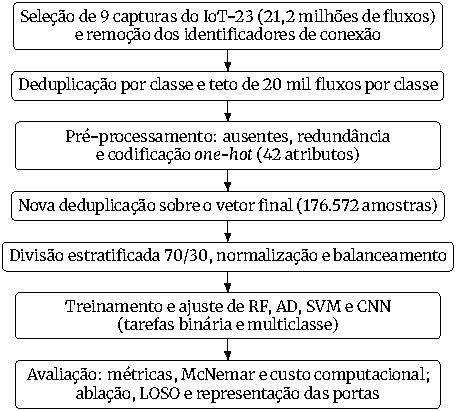
\includegraphics{figuras/fluxograma_metodologia.pdf}
\caption{Etapas da metodologia.}
\label{fig:metodo}
\end{figure}

% ---------------------------------------------------------------------
\subsection{Ferramentas}

Os experimentos foram implementados em Python 3.13, em um \textit{notebook} executado no Google Colab com GPU NVIDIA T4, com os dados e os modelos armazenados no Google Drive. Foram utilizadas as bibliotecas Pandas 2.2 e PyArrow, para manipulação dos dados; Scikit-learn 1.6 \citep{pedregosa2011scikit}, para RF, AD, SVM, busca de hiperparâmetros e métricas; imbalanced-learn 0.14 \citep{lemaitre2017imbalanced}, para o SMOTE; Keras com TensorFlow 2.20 \citep{abadi2016tensorflow}, para a CNN; statsmodels 0.15 \citep{seabold2010statsmodels}, para o teste de McNemar; e Matplotlib e Seaborn, para as visualizações.

% ---------------------------------------------------------------------
\subsection{Seleção dos cenários}

Foram utilizados os registros de conexão (\texttt{conn.log.labeled}) de nove capturas do IoT-23, apresentadas na \autoref{tab:cenarios}: seis cenários maliciosos, que contemplam as classes de ataque mais frequentes no conjunto (varredura de portas, Okiru e DDoS), além das classes de comando e controle e de ataque direto, e as três capturas benignas, obtidas de dispositivos reais em ambiente de \textit{honeypot}. As capturas maliciosas também contêm tráfego benigno, gerado pelos próprios dispositivos infectados. Na captura 36-1, foram descartados os fluxos com o rótulo residual \textit{Okiru-Attack}. No total, foram reunidos 21.223.743 fluxos. Ao longo do texto, a classe \textit{PartOfAHorizontalPortScan} é referida como \textit{portscan}.

\begin{table}[htbp]
\centering
\caption{Capturas do IoT-23 utilizadas \citep{garcia2020iot23}.}
\label{tab:cenarios}
\small
\setlength{\tabcolsep}{4pt}
\begin{tabular}{l>{\raggedright\arraybackslash}p{0.27\columnwidth}>{\raggedright\arraybackslash}p{0.30\columnwidth}r}
\toprule
\textbf{Captura} & \textbf{Malware / dispositivo} & \textbf{Classes maliciosas} & \textbf{Fluxos} \\
\midrule
1-1  & Hide and Seek & Portscan               &  1.008.748 \\
3-1  & Muhstik       & Attack, portscan       &    156.103 \\
8-1  & Hakai         & C\&C                   &     10.403 \\
9-1  & Hajime        & Portscan               &  6.378.293 \\
34-1 & Mirai         & DDoS, C\&C, portscan   &     23.145 \\
36-1 & Okiru         & Okiru, C\&C-HeartBeat  & 13.645.095 \\
\midrule
4-1  & Philips Hue (\textit{honeypot})  & -- & 452 \\
5-1  & Amazon Echo (\textit{honeypot})  & -- & 1.374 \\
7-1  & Somfy (\textit{honeypot})        & -- & 130 \\
\bottomrule
\end{tabular}
\end{table}

Já na leitura dos registros, foram descartados os atributos que identificam a conexão ou o momento em que ela ocorreu --- o carimbo de tempo, o identificador do fluxo e os endereços IP --- além de \texttt{tunnel\_parents}, uma vez que poderiam levar o modelo a memorizar dispositivos ou instantes específicos de cada captura, caracterizando vazamento de informação.

% ---------------------------------------------------------------------
\subsection{Deduplicação e amostragem}
\label{sec:dedup}

A análise exploratória revelou que o IoT-23 apresenta um grau extremo de repetição. Como mostra a \autoref{tab:dedup}, os 13,6 milhões de fluxos da classe Okiru correspondem a apenas 621 combinações distintas de atributos, e os 14.394 fluxos de DDoS, a apenas 224. Se o conjunto for dividido sem tratamento, cópias de um mesmo fluxo acabam no treino e no teste, e o modelo é avaliado sobre exemplos já vistos, o que constitui uma forma de vazamento de informação \citep{kapoor2023leakage}.

Por esse motivo, ainda sobre os atributos originais, os fluxos repetidos foram removidos dentro de cada classe e, somente depois, aplicou-se um teto de 20.000 fluxos por classe, por amostragem aleatória, para limitar o custo computacional; a classe benigna foi mantida integralmente. A ordem é relevante: amostrando antes de deduplicar, a classe Okiru era reduzida a apenas dois padrões distintos.

\begin{table}[htbp]
\centering
\caption{Fluxos por classe antes e depois da deduplicação por classe e do teto de amostragem.}
\label{tab:dedup}
\small
\begin{tabular}{lrrr}
\toprule
\textbf{Classe} & \textbf{Brutos} & \textbf{Únicos} & \textbf{Usados} \\
\midrule
Okiru           & 13.626.744 &     621 &     621 \\
Portscan        &  7.040.929 & 506.382 &  20.000 \\
Benigno         &    505.082 & 123.538 & 123.538 \\
C\&C-HeartBeat  &     15.688 &  15.687 &  15.687 \\
C\&C            &     14.944 &  10.827 &  10.827 \\
DDoS            &     14.394 &     224 &     224 \\
Attack          &      5.962 &   5.962 &   5.962 \\
\bottomrule
\end{tabular}
\end{table}

% ---------------------------------------------------------------------
\subsection{Pré-processamento}

Os atributos \texttt{local\_orig} e \texttt{local\_resp}, vazios em todos os fluxos, foram removidos. Para os atributos numéricos que ficam ausentes quando a conexão não é estabelecida (duração e bytes trocados), foi criado um indicador binário de ausência antes do preenchimento com zero, enquanto os categóricos \texttt{service} e \texttt{history} receberam a categoria ``desconhecido''.

A análise exploratória mostrou correlação praticamente perfeita entre os atributos \texttt{*\_ip\_bytes} e \texttt{*\_bytes}, e os primeiros foram removidos por redundância. As categorias de \texttt{history} com menos de 500 ocorrências foram agrupadas, e os atributos \texttt{proto}, \texttt{service}, \texttt{conn\_state} e \texttt{history} foram codificados por \textit{one-hot}. Ao final, cada fluxo passou a ser descrito por 42 atributos. As portas de origem e destino foram mantidas como atributos numéricos, como no trabalho de base \citep{souza2024avaliacao}; o efeito dessa escolha é investigado na \autoref{sec:res-portas} (AJUSTAR).

Como o pré-processamento torna idênticos alguns fluxos originalmente distintos, a deduplicação foi repetida sobre o vetor final de atributos, resultando em 176.572 amostras. A ausência de sobreposição entre treino e teste foi verificada pela comparação de \textit{hashes} dos vetores de atributos.

% ---------------------------------------------------------------------
\subsection{Divisão, normalização e balanceamento}

Os experimentos foram conduzidos em uma tarefa \textbf{binária} (benigno ou malicioso) e em uma tarefa \textbf{multiclasse}, com as sete classes da \autoref{tab:dedup}. O conjunto foi dividido em 70\% para treino (123.600 amostras) e 30\% para teste (52.972 amostras), de forma estratificada pelo rótulo multiclasse, e a tarefa binária utiliza a mesma divisão. Os atributos numéricos foram padronizados com média zero e desvio padrão unitário, com parâmetros calculados apenas sobre o treino.

Para lidar com o desbalanceamento --- no treino multiclasse, a classe benigna tem 86.300 amostras, e as classes Okiru e DDoS, apenas 435 e 156 ---, todos os modelos utilizaram ponderação de classes inversamente proporcional à frequência (\texttt{class\_weight='balanced'}). O SMOTE \citep{chawla2002smote} foi testado apenas na tarefa binária, em comparação com a ponderação de classes, já que, na multiclasse, a interpolação entre os poucos padrões distintos de Okiru e DDoS não acrescentaria informação real.

% ---------------------------------------------------------------------
\subsection{Modelos e ajuste de hiperparâmetros}

Para a CNN, cada vetor de 42 atributos foi reorganizado em uma matriz $6 \times 7$, sem necessidade de \textit{zero-padding}. A arquitetura é composta por duas camadas convolucionais com ativação ReLU, uma camada de \textit{max pooling} $2 \times 2$, uma camada densa com \textit{dropout} e a camada de saída \textit{softmax}. O treinamento utilizou a entropia cruzada categórica como função de perda e o otimizador Adam, com no máximo 150 épocas e parada antecipada (\textit{early stopping}) após 10 épocas sem melhora da perda na validação. O SVM utilizou núcleo RBF. A semente aleatória foi fixada em 42, exceto nas execuções repetidas da CNN (\autoref{sec:avaliacao}).

O ajuste de hiperparâmetros utilizou o F1-macro como critério, sem uso do conjunto de teste. Para RF, AD e SVM, foi feita busca em grade (\textit{Grid Search}) com validação cruzada estratificada de 5 \textit{folds}. No caso do SVM, devido ao maior custo de treinamento, a busca foi realizada em uma subamostra estratificada de cerca de 20 mil amostras, na qual a classe benigna foi reduzida; por isso, o F1-macro foi calculado com pesos que restituem a proporção real das classes no treino. Para a CNN, foram avaliadas oito configurações sorteadas (\textit{Random Search}), usando 20\% do treino como validação. Os espaços de busca e as configurações selecionadas estão na \autoref{tab:hiper}. Os valores escolhidos para o SVM ficaram no limite superior da grade, de modo que o melhor ajuste pode estar além da região explorada, o que constitui uma limitação deste trabalho.

\begin{table}[htbp]
\centering
\caption{Espaços de busca e hiperparâmetros selecionados (binária / multiclasse); $\gamma_0 \approx 0{,}061$ é o valor padrão da biblioteca.}
\label{tab:hiper}
\small
\setlength{\tabcolsep}{3pt}
\begin{tabular}{l>{\raggedright\arraybackslash}p{0.47\columnwidth}>{\raggedright\arraybackslash}p{0.33\columnwidth}}
\toprule
\textbf{Modelo} & \textbf{Espaço de busca} & \textbf{Selecionado} \\
\midrule
RF  & árvores $\in \{50, 100, 200\}$; profundidade $\in \{$sem limite$, 10, 20\}$ & 100 / 200 árvores, sem limite \\
\midrule
AD  & critério $\in \{$Gini, entropia$\}$; profundidade $\in \{$sem limite$, 5, 10, 20\}$; folha mínima $\in \{1, 5\}$ & Gini, profundidade 20, folha 1 \\
\midrule
SVM & $C \in \{10, 100, 1000\}$; $\gamma \in \{\gamma_0, 4\gamma_0, 16\gamma_0\}$ & $C = 1000$, $\gamma = 16\,\gamma_0$ \\
\midrule
CNN & filtros $\in \{(16,32), (32,64), (64,128)\}$; núcleo $\in \{2, 3\}$; densa $\in \{64, 128, 256\}$; \textit{dropout} $\in \{0{,}2;\,0{,}3;\,0{,}5\}$; taxa $\in \{10^{-3},\,3 \cdot 10^{-4}\}$; lote $\in \{256, 512\}$ & (32,64), núcleo 2, densa 128, taxa $10^{-3}$; \textit{dropout} 0,3 / 0,5; lote 256 / 512 \\
\bottomrule
\end{tabular}
\end{table}

% ---------------------------------------------------------------------
\subsection{Protocolo de avaliação}
\label{sec:avaliacao}

Os modelos finais foram avaliados no conjunto de teste pela acurácia e pela precisão, \textit{recall} e F1-Score em média macro, sendo o \textbf{F1-macro} o critério principal, e pelo tempo de inferência por amostra, medido em CPU. A estabilidade dos resultados foi verificada por validação cruzada de 5 \textit{folds} no treino, para RF, AD e SVM, e, para a CNN, por cinco execuções com as sementes 42, 7, 123, 2024 e 31415; nas análises seguintes, utilizou-se a execução da CNN com F1 mediano. A importância dos atributos foi estimada pela redução média de impureza (MDI) do RF multiclasse.

As diferenças entre os modelos foram avaliadas pelo teste de McNemar exato (\autoref{sec:rev-metricas} AJUSTAR), aplicado par a par sobre as predições no conjunto de teste, nas duas tarefas. O teste considera apenas se cada modelo acertou ou errou cada amostra, o que permite aplicá-lo da mesma forma às tarefas binária e multiclasse. Como são seis comparações por tarefa, adotou-se a correção de Bonferroni, com nível de significância $\alpha = 0{,}05/6 \approx 0{,}0083$.

Além da avaliação convencional, foram realizados três experimentos complementares:
\begin{itemize}
    \item \textbf{Ablação da deduplicação}: o RF binário foi treinado também sem a segunda deduplicação e sem nenhuma deduplicação, etapa não descrita no trabalho de base, para medir o efeito da repetição dos fluxos. Nesta última condição, o teto de 20.000 fluxos passou a valer também para a classe benigna;
    \item \textbf{\textit{Leave-one-scenario-out} (LOSO)}: cada uma das seis capturas maliciosas foi, por vez, retirada do treino e usada como teste, junto com 30\% dos fluxos de \textit{honeypot}, sempre os mesmos; os 70\% restantes integraram o treino. Assim, cada rodada simula a chegada de tráfego de uma captura nunca vista, com outro malware, outro dispositivo e outra rede. Em três rodadas (3-1, 34-1 e 36-1), o teste contém classes de ataque ausentes do treino; nas demais, a classe já é conhecida, mas provém de outra captura. Os modelos foram retreinados com os mesmos hiperparâmetros, e mediu-se a \textbf{taxa de detecção}, ou seja, a porcentagem dos fluxos maliciosos da captura classificados como maliciosos, e a taxa de falsos positivos nos fluxos benignos da própria captura;
    \item \textbf{Representação das portas}: motivado pela importância das portas no RF, avaliou-se o efeito de removê-las dos atributos, nos modelos de árvore, e de codificá-las como categorias, na CNN. Nesse caso, cada porta com ao menos 500 ocorrências no treino (15 de destino e 4 de origem) recebeu uma coluna \textit{one-hot}, mais uma categoria ``outras'' por atributo, o que elevou a entrada para 61 atributos, organizados em uma matriz $7 \times 9$ com \textit{zero-padding}. O SVM não foi incluído neste experimento devido ao custo computacional.
\end{itemize}

%%%%%%%%%%%%%%%%%%%%%%%%%%%%%%%%%%%%%%%%%%%%%%%%%%%%%%%%%%%%%%
%%%%%%%% SEÇÃO 4 RESULTADOS (4.1 a 4.6)
%%%%%%%%%%%%%%%%%%%%%%%%%%%%%%%%%%%%%%%%%%%%%%%%%%%%%%%%%%%%%%

% =====================================================================
\section{Resultados e discussão}
\label{sec:resultados}

AJUSTAR

%%%%%%%%%%%%%%%%%%%%%%%%%%%%%%%%%%%%%%%%%%%%%%%%%%%%%%%%%%%%%%
%%%%%%%% SEÇÃO 5 CONSIDERAÇÕES FINAIS
%%%%%%%%%%%%%%%%%%%%%%%%%%%%%%%%%%%%%%%%%%%%%%%%%%%%%%%%%%%%%%

% =====================================================================
\section{Considerações finais}
\label{sec:conclusao}

AJUSTAR

\bibliography{referencias}

\end{document}